% This is samplepaper.tex, a sample chapter demonstrating the
% LLNCS macro package for Springer Computer Science proceedings;
% Version 2.21 of 2022/01/12
%
\documentclass[runningheads]{llncs}
%
\usepackage[T1]{fontenc}
% T1 fonts will be used to generate the final print and online PDFs,
% so please use T1 fonts in your manuscript whenever possible.
% Other font encondings may result in incorrect characters.
%
\usepackage{graphicx}
% Used for displaying a sample figure. If possible, figure files should
% be included in EPS format.
%
% If you use the hyperref package, please uncomment the following two lines
% to display URLs in blue roman font according to Springer's eBook style:
%\usepackage{color}
%\renewcommand\UrlFont{\color{blue}\rmfamily}
%

\usepackage[a4paper,margin=2.5cm]{geometry}

\usepackage[%
  backend=biber,
  url=false,
  style=numeric, % alphabetic, numeric
  maxnames=4,
  minnames=3,
  maxbibnames=99,
  giveninits,
  uniquename=init]{biblatex}

\bibliography{bibliography}

\begin{document}
%
\title{Formal Software Verification Project Report\newline{}SAT Solver}
%
\titlerunning{FSV Project Report}
% If the paper title is too long for the running head, you can set
% an abbreviated paper title here
%
\author{Nathan Schmidt}
%
\authorrunning{N. Schmidt}
% First names are abbreviated in the running head.
% If there are more than two authors, 'et al.' is used.
%
\institute{Aarhus University, Aarhus, Denmark\\
Student number: 202400801}
%
\maketitle              % typeset the header of the contribution
%
\begin{abstract}
The abstract should briefly summarize the contents of the paper in
150--250 words.

% \keywords{First keyword  \and Second keyword \and Another keyword.}
\end{abstract}
%
%
%

\section{Introduction}\label{sec:intro}

The \emph{Boolean Satisfiability Problem (SAT)} consists in determining whether, given a formula of propositional logic, there exists a \emph{valuation} that satisfies it, i.e., a mapping from the unknowns of the formula to boolean values such that the formula holds. 
Great numbers of problems in computer science can easily be reduced to SAT, and even though SAT is known to be $\mathcal{NP}$-complete by the Cook-Levin theorem of 1971 \cite{cook1971} and its many proofs since then, there exist many efficient \emph{SAT-Solvers} for certain classes of formulas.

\bigbreak

In this project, we implement a small formally verified SAT-Solver in the \textsc{Coq} proof assistant for formulas containing conjunctions, disjunctions, implications, and negations. 
To that end, we start by formalizing the syntax of such formulas. 
Then, we introduce their semantic interpretation given a specified valuation. 
Following the implementation of a syntactic optimizer that we show to simplify a formula to its minimal form, we conclude this work by implementing the actual solver based on a brute-force search algorithm and prove it to be both correct and complete.
\section{Implementation and Encountered Problems}\label{sec:impl}

In this section, we present our implementation choices and compare them to discarded alternatives to justify them. 
We also describe what difficulties we encountered during development and how we addressed them.

\subsection{Syntax}

First, we formalize the abstract syntax of boolean formulas containing conjunctions, disjunctions, implications, and negations. 

\subsubsection{Abstract Syntax.}

We state an inductive definition of the type \texttt{form} with a set of constructors describing how to build up a formula:
\begin{equation}
    p, q ::= x\;|\;\texttt{true}\;|\;\texttt{false}\;|\;p \land q\;|\;p \lor q\;|\;p \rightarrow q\;|\;\neg p
\end{equation}

For identifiers, we introduce the type \texttt{id} with a single constructor \texttt{Id} that wraps a string. 
We also define an equality function comparing two identifiers and returning \texttt{true} if and only if their contained strings are equal. To ease proof development in the rest of the project, we prove some basic lemmas and theorems about the function by case distinction, namely \emph{reflexivity}, \emph{equivalence with propositional equality}, and \emph{decidability} of equality of identifiers.
For the decidability theorem, one needs to ensure its proof is concluded by \texttt{Defined.} instead of \texttt{Qed.} as its proof object is needed in the computation of later used functions and thus has to be saved.

\subsubsection{Concrete Syntax.}

To make reading and writing formulas easier, we use \textsc{Coq}'s \texttt{Notation}s system, as well as a \texttt{Coercion} from an identifier as a formula. 
The main difficulty lies in assigning precedence levels to the individual constructors that pay respect to the commonly assumed binding of operators. 
Given the \emph{binds stronger} relation ($>$), that is:
\begin{equation}
    \neg > \land > \lor >\,\rightarrow
\end{equation}
For example, $x \lor \neg y \land z \rightarrow \texttt{false}$ is interpreted as $(x \lor ((\neg y) \land z) \rightarrow \texttt{false}$. 

\subsection{Semantics}

Now that we can write a formula in \textsc{Coq}, we want to define its semantics, i.e., if we interpret it as \texttt{true} or \texttt{false}.

\subsubsection{Valuations.} % TODO: clarify valuation notation

To do so, we need to know which boolean values to replace all identifiers occurring in a formula with.
Therefore, we define the type \texttt{valuation}. 
A \emph{valuation} is a function that, being passed an identifier, returns \texttt{true} or \texttt{false}, or, in other words, a valuation is a total map from identifiers to booleans. 
Our implementation is analogous to the total map defined by Pierce et al. in \cite{pierceSF}.
% An empty valuation is a valuation that returns \texttt{false} for all arguments.

Again, to simplify writing and reading valuations, we introduce a \texttt{Notation} \texttt{x !-> b ;; v} to override a valuation \texttt{v} with a new value \texttt{b} for \texttt{x}. 
At first, we used just a single semicolon, but this caused conflicts with list notations. 
Additionally, we define an empty valuation to map all identifiers to \texttt{false}.

We also specify some lemmas of \cite{pierceSF} for later reasonings. 
Their proofs rely on the functional extensionality axiom, stating that two functions are equal if and only if their applications to all their possible arguments are equal. 
It is known to be compatible with \textsc{Coq}'s logical core.

\subsubsection{Interpreter.}

The \texttt{valuation} type allows us to define a recursive interpretation function \texttt{interp}.
Applied to a valuation and a formula, it returns \texttt{true} if and only if the formula holds by traversing a formula bottom-up and pattern matching on it.
All the necessary functions, such as \texttt{andb}, \texttt{orb}, and \texttt{negb} are already implemented in \textsc{Coq}. 
They even suffice to compute the result of an implication since $p \rightarrow q$ is known to be equivalent to $\neg p \lor q$.

\subsection{Optimizer}

Sometimes, a formula's interpretation can be derived or, at least, simplified on a purely syntactical level, leaving it in a form that is easier to read and reason upon and marginally reducing the computation effort needed by the interpretation function while preserving the semantics.
In this part of the project, we therefore introduce an optimization function \texttt{optim}.

\subsubsection{Minimality.}

A key challenge was formally defining what a simplification is and what property the result of \texttt{optim} should have.

A \emph{simplification} reduces the applications of the binary operators $\land$, $\lor$ and $\rightarrow$ to one of their two arguments or an \emph{atom}, i.e., the boolean values \texttt{true} and \texttt{false}. 
Additionally, when applied to an atom, the unary operation $\neg$ can be simplified to an atom.

The aim is to leave a formula $p$ in a form that cannot be simplified further on a syntactical level.
We assume this to be the case in exactly two mutually exclusive situations:
\begin{itemize}
    \item $p$ is an atom, or
    \item $p$ does not contain any atoms.
\end{itemize}
When one of the situations applies, we say $p$ is in \emph{minimal form}. Formalizing this definition in \textsc{Coq}, we require either a fixpoint returning \texttt{true} if and only if a formula does not contain atoms or an inductive proposition.
While we initially opted for a fixpoint, proving the correctness of our optimizer later turned out easier with an inductive proposition. 
A formula does not contain an atom if it is an identifier or if all its subformulas do not contain atoms.

We settle on a set of laws that our optimizer uses and allow it to fulfill the above-mentioned correctness and minimality requirements:
\begin{alignat}{4}
    \texttt{true} \land p &\equiv p &p \land \texttt{true} &\equiv p &\texttt{false} \land p &\equiv \texttt{false}\hspace*{20pt}&p \land \texttt{false} &\equiv \texttt{false} \\
    \texttt{true} \lor p &\equiv \texttt{true}\hspace*{20pt}&p \lor \texttt{true} &\equiv \texttt{true}\hspace*{20pt}&\texttt{false} \lor p &\equiv p &p \lor \texttt{false} &\equiv p \\
    \texttt{true} \rightarrow p &\equiv p &p \rightarrow \texttt{true} &\equiv \texttt{true} &\texttt{false} \rightarrow p &\equiv \texttt{true} &p \rightarrow \texttt{false} &\equiv \neg p \\
    &&\neg \texttt{true} &\equiv \texttt{false} &\neg \texttt{false} &\equiv \texttt{true}
\end{alignat}

Note that we leave out some further simplification potential. 
For improved provability, we only concentrate on laws involving at least one atom.
One could also go beyond and, e.g., add laws such as $p \land \neg p \equiv \texttt{false}$ for an arbitrary formula $p$ to this set.

\subsubsection{Implementation.}

The actual implementation of the optimizer in \textsc{Coq} requires a bit of thought.
Indeed, our first implementation attempt was a top-down traversal of the abstract syntax tree of the given formula and successive application of the listed simplifications.
However, this misses some optimization potential as it may only become available after optimizing subformulas.
To try and remedy this, we wrote a recursive function repeatedly applying \texttt{optim} on a formula until reaching a fixpoint.
While a fixpoint is eventually reached in practice, \textsc{Coq} cannot know and rejects the function as new arguments to \texttt{optim} are not obviously smaller.

\begin{figure}[t]
    \centering
    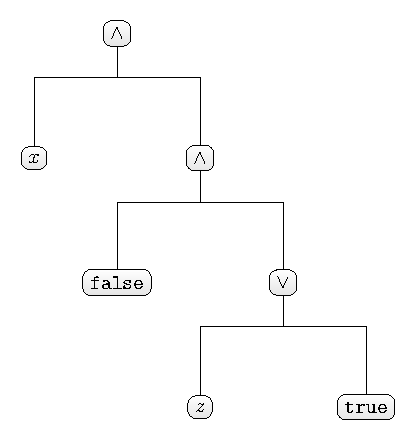
\includegraphics[scale=0.82,valign=t]{figures/optimizer1.pdf}
    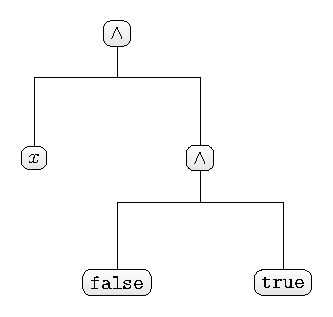
\includegraphics[scale=0.82,valign=t]{figures/optimizer2.pdf}
    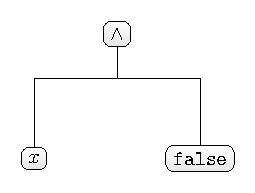
\includegraphics[scale=0.82,valign=t]{figures/optimizer3.pdf}
    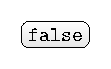
\includegraphics[scale=0.82,valign=t]{figures/optimizer4.pdf}
    \caption{Successive syntactical optimization steps on $x \land (\texttt{false} \land (z \lor \texttt{true}))$.}
    \label{fig:optimizer}
\end{figure}

Instead, our revised approach only traverses the passed formula once and hence only requires linear runtime.
We achieve this by performing a post-order depth-first-search (DFS) on the abstract syntax tree of the passed formula.
This way, optimizations of subformulas are directly taken into account.
Even though sometimes it is sufficient to simplify only one or even no subformula, we always traverse the whole tree for easier proving of the required properties.
Figure \ref{fig:optimizer} illustrates such a case, where for the formula $x \land (\texttt{false} \land (z \lor \texttt{true}))$, the subformula $z \lor \texttt{true}$ is simplified to \texttt{true} first, even though $\texttt{false} \land (z \lor \texttt{true})$ could directly be simplified to \texttt{false} from the get-go.
Note, however, that the formula is translated to \texttt{false} without even running the interpreter just by its syntax.

\subsubsection{Properties.}

To close off this section, we must formally verify that our optimizer truly meets its requirements.
First and foremost, the following theorem holds:
\begin{theorem}
    For all valuations $v$ and formulas $p$, $\texttt{interp}\;v\;p = \texttt{interp}\;v\;(\texttt{optim}\;p)$, i.e., the optimizer is correct since it preserves the semantics of formulas.
\end{theorem}
\begin{proof}
    We proceed by induction on the structure of $p$. 
    The non-trivial cases $p = q_1 \land q_2$, $p = q_1 \lor q_2$ and $p = q_1 \rightarrow q_2$ are all shown by case distinction on $\texttt{optim}\;q_1$ and $\texttt{optim}\;q_2$ and application of the induction hypotheses claiming the optimizer is correct for $q_1$ and $q_2$.
    $p = \neg q$ follows the same pattern for a single subformula $q$. \qed
\end{proof}
The main challenges for formally proving this theorem in \textsc{Coq} do not lie in the reasoning but rather in removing redundancies.
Consequently, as for many other proofs of the project, we decided to first write a mostly manually written version before looking out for automation potential.
In a final step, we filtered out common patterns through custom tactics through the \texttt{Ltac} language. 

We also prove this second theorem to show our optimizer is actually exhaustive:
\begin{theorem}
    For all formulas $p$, the result of the optimizer $\texttt{optim}\;p$ is in minimal form.
\end{theorem}
\begin{proof}
    We proceed by induction on the structure of $p$.
    For the cases $p = q_1 \land q_2$, $p = q_2 \lor q_2$, $p = q_1 \rightarrow q_2$ and $p = \neg q$, we perform case distinctions on the induction hypotheses (minimality of the subformulas), as well as the results of the optimizer applied to them.
    If necessary, we invert the induction hypotheses involving the deconstructed optimizer results.
    Then, it follows directly from the hypotheses set that $p$ either does not contain atoms or, on the contrary, is an atom. \qed
\end{proof}
For this \textsc{Coq} proof, many cases are very similar, but, e.g., differ in the actual atom $p$ is equal to, reducing the potential for automation, as one must carefully introduce a fitting witness for the left branch of minimality, i.e., \texttt{exists b, p = form\_bool b}.
Nevertheless, we factor out the recurrent patterns of deconstructing and rewriting with the induction hypotheses and destructing $\texttt{optim}\;q$ for a subformula $q$ and then inverting one of the induction hypotheses. In some rare cases, some forms are shelved in the process, requiring the use of \texttt{Unshelve}, which we were unaware of beforehand.

\subsection{Solver}

In this section, we can finally deal with our SAT solver.
Our idea is to collect representatives for all classes of valuations that are susceptible of satisfying a given formula and test them on the formula until one positive interpretation is found or no valuation matches.
Indeed, only identifiers that are in a formula influence its interpretation, and we can safely map all identifiers not contained in a formula to \texttt{false} in our collected valuations:
\begin{lemma}
    For any formula, two otherwise identical valuations differing in the value of an identifier that is not contained in the formula lead to an identical interpretation.
\end{lemma}

Initially, we wanted to write a function that directly collects all relevant valuations for a given formula.
While this is possible, it would have inevitably collected duplicate valuations as comparing valuations is not computable, as valuations are, in turn, functions themselves.
Duplicate valuations can, however, lead to a significantly increased runtime of our solver in some cases.
For instance, consider the unsatisfiable formula $x \land \neg x$.
The initial function would collect \texttt{[$x$ !-> true ; $x$ !-> true ; empty\_valuation]}.
We would then check the valuation \texttt{$x$ !-> true} twice, even though it does not satisfy the formula.
Generalized to examples with many duplicate identifiers in respective subformulas, this does not scale.

\begin{figure}[t]
    \centering
    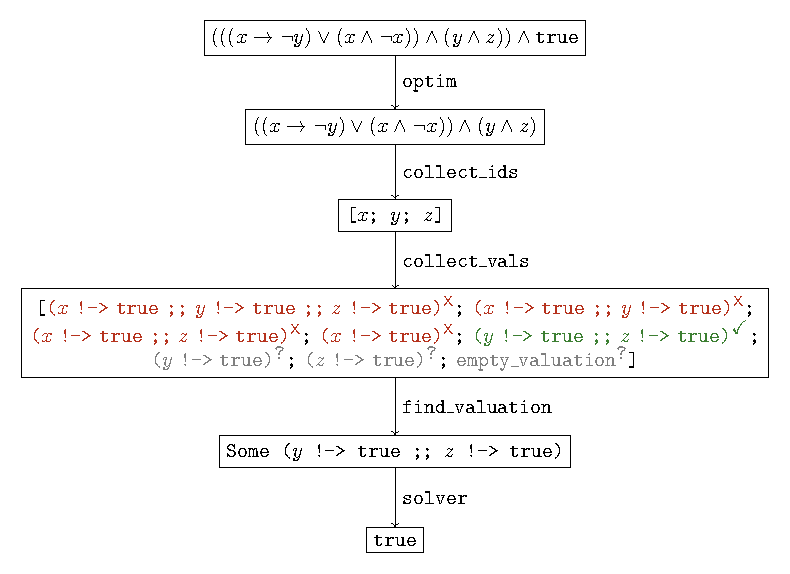
\includegraphics[scale=0.9]{figures/solver.pdf}
    \caption{Exemplary solving process for $(((x \rightarrow \neg y) \lor (x \land \neg x)) \land (y \land z)) \land \texttt{true}$.}
    \label{fig:solver}
\end{figure}

Instead, we decide to implement our solver with three individual functions.
We name them explicitly rather than defining them as anonymous fixpoints and can hence show some detached properties in \textsc{Coq}.
Throughout this section, we will use the formula $(((x \rightarrow \neg y) \lor (x \land \neg x)) \land (y \land z)) \land \texttt{true}$ as running example to illustrate the solving steps as depicted in figure \ref{fig:solver}.

\subsubsection{Extracting Identifiers.}

To tackle the above-mentioned problem, we provide a dedicated recursive function \texttt{collect\_ids} that collects all identifiers of a formula without duplicates (compare example in figure \ref{fig:solver}).

\begin{figure}[t]
    \begin{lstlisting}[language=coq,numbers=left,numberstyle=\tiny,label=lst:ids_union,caption=Custom duplicate free list merging function.]
Fixpoint ids_union (l1 l2 : list id) : list id :=
  match l1 with
  | [] => l2
  | x::xs => if existsb (eqb_id x) l2 then ids_union xs l2 else ids_union xs (x :: l2)
  end.
    \end{lstlisting}
\end{figure}

We wanted the result of the function to be a finite set but did not find a standard library implementation that fully corresponded to our expectations.
Thus, we first decided to return a list and take care ourselves to not include any duplicates.
The abandoned implementation of a function merging the lists of collect identifiers of two subformulas without duplicates can be found in listing \ref{lst:ids_union}.
We formally proved that elements included in either \texttt{l1} or \texttt{l2} are all kept in the result, that any element of the result is originally contained in \texttt{l1} or \texttt{l2}, and that if \texttt{NoDup l1} and \texttt{NoDup l2}, then \texttt{NoDup (ids\_union l1 l2)} holds.

After some deeper search through the standard library, we, in the end, opted for the finite set implementation provided in \texttt{Coq.Lists.ListSet}\footnote{\url{https://coq.inria.fr/doc/v8.9/stdlib/Coq.Lists.ListSet.html}}.
Even though it does not hide many implementation details, it comes with some predefined set manipulation operations and some lemmas about its properties, which would not have justified a similar custom re-implementation.
To confirm it matches our expectations, we show that \texttt{set\_add} behaves as the identity function if we try adding an identifier $x$ to a set that already contains it and that it behaves as an append of the one-element list \texttt{[$x$]} to the end of the set, which in fact is just a list, else.

The most relevant property of \texttt{collect\_ids} is however the following:
\begin{lemma}
    An identifier is contained in a formula $p$ if and only if it is contained in \texttt{collect\_ids\;$p$}.
\end{lemma}
\begin{proof}
    We consider the forward ($\Longrightarrow$) and backward ($\Longleftarrow$) directions separately.
    For both directions, the proof of the statement by induction on $p$ is fairly straightforward.
    \begin{itemize}
        \item In the forward direction, the conjunction, disjunction, and implication cases require a deconstruction of the hypothesis stating that some arbitrary but fixed identifier is contained in at least one subformula.
        We can then show that identifiers of subformulas are preserved using our induction hypotheses.
        \item The backward direction is analogous, using the fact that an identifier contained in the union of two sets is contained in at least one of the two sets. \qed
    \end{itemize}
\end{proof}
While the proof simply requires a case distinction on our hypothesis and applying the relevant induction hypothesis for the inductive cases, the main difficulty was finding and plugging in relevant standard library lemmas when needed, avoiding proving already known facts.
Other than that, the formal proof contained a lot of repetition, and we were able to significantly shorten it using \texttt{Ltac} for a common pattern of deconstruction followed by application and a succession of \texttt{try} tactics.

\subsubsection{Collecting Valuations.}

As we now have the ability to collect the identifiers of formulas, we need to transform identifier sets into a list of all relevant valuations that could satisfy this formula.
We hence introduce the \texttt{collect\_vals} function.
Its implementation maps each identifier of the passed set to \texttt{true} on top of the already collected valuations, which are already kept.
One does not need to explicitly map identifiers to \texttt{false} since the function returns the empty valuation for the empty set, which maps all identifiers to \texttt{false}, and is hence always included in the resulting list (which we formally prove in \textsc{Coq}).

\begin{figure}[t]
    \begin{lstlisting}[language=coq,numbers=left,numberstyle=\tiny,escapeinside={€}{€},label=lst:old-collect_vals,caption=Original tail-recursive valuation collection function.]
Fixpoint collect_vals (l : list id) (acc : list valuation) : list valuation :=
  match l with
  | [] => acc
  | x::xs => collect_vals xs ((map (fun v => x !-> true ;; v) acc) €\texttt{++}€ (map (fun v => x !-> false ;; v) acc))
  end.
    \end{lstlisting}
\end{figure}

Initially, we implemented a tail-recursive version of the function based on an accumulator element as depicted in listing \ref{lst:old-collect_vals}.
When called with \texttt{[empty\_valuation]} as starting accumulator, the function yields the desired result.
However, while this allows code optimizations as all calls to the function are last, it complicates proving properties as some assumptions on the accumulator are required.
This illustrates the often encountered trade-off between efficiency considerations of smart implementations and proof complexity.
Additionally, we suspected at first that explicitly mapping newly added identifiers to \texttt{false} would make some proofs easier, but the opposite turned out to be the case.

To verify the \texttt{collect\_vals} correctly includes valuations for both truth values of every identifier contained in the passed finite set, we prove we formally prove the following lemma in \textsc{Coq}:
\begin{lemma}
    For all identifier sets $S$, any $x \in S$ if and only if there exist valuations in \texttt{collect\_vals\;$S$} where $x$ is respectively mapped to \texttt{true} and \texttt{false}.
\end{lemma}
A significant part of the backward direction of this lemma was proven using a custom \texttt{Ltac} tactic. 
Still, as \texttt{Ltac} is only quickly tackled in the course, we lacked the knowledge to automatically derive witnesses from the list of assumptions.

\subsubsection{Searching Through Valuations.}

\begin{figure}[t]
    \begin{lstlisting}[language=coq,numbers=left,numberstyle=\tiny,escapeinside={€}{€},label=lst:alt-check_vals,caption=Alternative valuation search functions.]
Definition check_vals (p : form) (l : list valuation) : option valuation :=
  let l' := map (fun v => if interp v p then Some v else None) l in
  match find (fun o => match o with Some _ => true | None => false end) l' with
  | Some o => o
  | None => None
  end.

Definition check_vals' (p : form) (l : list valuation) : bool :=
  existsb (fun b => b) (map (fun v => interp v p) l).
    \end{lstlisting}
\end{figure}

The final solving step performed by \texttt{check\_vals} is to search through a list of valuations $l$ and return \texttt{Some $v$} if $v$, contained in $l$, satisfies the formula $p$.
It returns \texttt{None} if no valuation matches.
One considered option was to use the library function \texttt{map} to interpret all collected valuations on a formula, and then either \texttt{find} a matching valuation or, if the actually found valuation does not matter, return the first found \texttt{true} in the altered list.
Two possible implementations are shown in listing \ref{lst:alt-check_vals}.
Even though we avoid explicitly writing pattern matching and recursion, these options are both less efficient -- \texttt{interp} is applied to all valuations, not just the first satisfying the formula -- and complicate proofs, especially improving reliance on standard library lemmas.
Consequently, in our final version of the function, we just recurse over the list of valuations until the first match, which is returned.
Later valuations are not considered, as illustrated by our running example in figure \ref{fig:solver}.

Putting it all together, the function \texttt{find\_valuation} accepts a formula $p$ and returns the result of the successive applications of \texttt{optim}, \texttt{collect\_ids}, \texttt{collect\_vals}, and \texttt{check\_vals}.
Note that in the worst case, \texttt{find\_valuation} searches through all relevant valuations if no valuation satisfies the formula, leading to a worst-case complexity of $\mathcal{O}(n^2)$ with $n$ being the number of identifiers contained in the formula.
Indeed, this makes sense as \textbf{NP} $\subseteq$ \textbf{EXPTIME}. % TODO: rethink this

The function \texttt{solver} then connects the result of \texttt{find\_valuation} to booleans, i.e., returns \texttt{true} for \texttt{Some $v$} and \texttt{false} for \texttt{None}.
In other words, \texttt{solver} is a \emph{decision procedure} \cite{kroening2016decision} for the boolean satisfiability problem.
This means \texttt{solver} is an algorithm that, given a concrete formula $p$, can always answer the problem by yes (\texttt{true}) if $p$ is satisfiable, and by no (\texttt{false}) if it is not satisfiable.
We will deal with the formal proof of this claim in the remainder of this subsection.

\subsubsection{Soundness.}

First, we need to show that \texttt{solver} has no false positives, i.e., does not falsely claim a formula to be satisfiable that is not.
This gives rise to the \emph{soundness} lemma:
\begin{lemma}
    For all formulas $p$, if \texttt{solver $p$} returns \texttt{true}, then $p$ is satisfiable.
\end{lemma}
\begin{proof}
    Assume \texttt{solver $p$} to return \texttt{true}.
    This is only the case when \texttt{find\_valuation $p$} returns \texttt{Some $v$}.
    We show by induction on the length of the list $l =$ \texttt{collect\_vals (collect\_ids (optim $p$))} that \texttt{interp $v$ (optim $p$)} is true, from which our claim directly follows as \texttt{optim} is semantics-preserving and $v$ is our witness for the satisfiability of $p$.
    \begin{itemize}
        \item Base case: if $l = \texttt{[]}$, \texttt{find\_valuation $p$} must be \texttt{None}, a contradiction with our hypothesis.
        \item Inductive step: let $l = \texttt{$v'$::$vs$}$ and our induction hypothesis be \texttt{check\_vals (optim $p$) vs = Some $v \Longrightarrow$ interp $v$ $p$ = true}.
        If \texttt{interp $v'$ $p$ = true}, then $v' = v$, and thus \texttt{find\_valuation $p$} returns \texttt{Some $v$}.
        Otherwise, we can apply our induction hypothesis and our goal immediately follows from our hypothesis. \qed
    \end{itemize}
\end{proof}
This can be concisely formalized in \textsc{Coq}.
One needs to perform some careful unfoldings while not revealing the inner parts of \texttt{solver}: it is irrelevant which valuation is returned, just that some valuation is returned.
Only then should the induction be performed.

\subsubsection{Completeness.}

Showing the completeness of \texttt{solver} was the most challenging part of the project, which we unfortunately did not fully manage to wrap up.
Indeed, one cannot blindly apply induction as the hypothesis is not directly usable to prove the lemma, and it took us a lot of time to figure out a coherent reasoning, writing a lot of later unused and removed helper lemmas.

The hypothesis that a formula $p$ is satisfiable means a valuation $v$ exists such that \texttt{interp $v$ $p$} is \texttt{true}.
However, it is in no way guaranteed that this is the valuation that will be found by \texttt{find\_valuation}.
In fact, it cannot be shown at all that this valuation will be found as our solver only looks at a subset of all valuations.
The problem has its roots in valuations being total maps.
For instance, let $v$ satisfy the formula $x \lor y$.
It is perfectly possible for $v$ to map an identifier $z$ not contained in the formula to \texttt{true} as this does not influence the formula's interpretation.
This consequently means our solver will not consider this exact $v$, as all uncontained identifiers are mapped to \texttt{false}.

Consequently, we first have to deduce our solver will consider some \emph{equivalent} $v'$.
This requires a formalization of the notion of equivalence first:
\begin{lemma}
    For all valuations $v$, $v'$, and formulas $p$, if $v$ and $v'$ map all identifiers contained in $p$ to the same value, then the interpretation of $p$ under the context of these two valuations is identical.
\end{lemma}
The main difficulty for this lemma does not lie in its proof, which can be performed by induction on $p$, but in the careful translation of this statement in \textsc{Coq}.
One needs to note that
\begin{lstlisting}[language=coq]
forall (v v' : valuation) (p : form) (x : id),
    (id_in_form x p = true -> v x = v' x) -> interp v p = interp v' p
\end{lstlisting}
only means $v$ and $v'$ correspond in a single identifier, which naturally does not imply their interpretations to be identical.
We rather need to nest the universal quantifier for $x$ as follows:
\begin{lstlisting}[language=coq]
forall (v v' : valuation) (p : form),
    (forall (x : id), id_in_form x p = true -> v x = v' x) -> interp v p = interp v' p
\end{lstlisting}
This nesting is, however, what will later lead our reasoning for the correctness proof not to be formalizable in \textsc{Coq}.

Now, we want to prove that \texttt{find\_valuation} will truly consider a valuation $v'$ equivalent to the known satisfying valuation $v$:
\begin{lemma}\label{lem:collect_equiv_v}
    For all valuations $v$ and formulas $p$, there exists a valuation $v'$ such that $v$ and $v'$ map all identifiers contained in $p$ to the same value and $v'$ is in \texttt{collect\_vals (collect\_ids $p$))}.
\end{lemma}
To formally show this in \textsc{Coq}, we first have to prove that \texttt{collect\_vals} preserves valuations when performing the union of identifier sets, i.e., if a valuation is contained in \texttt{collect\_vals $S$}, then it is also contained in \texttt{collect\_vals (id\_set\_union $S$ $S'$)} and in \texttt{collect\_vals (id\_set\_union $S'$ $S$)} for some second set $S'$.
Additionally, we also show that arbitrary combinations of valuations $v \in S$ and $v' \in S'$ are contained in \texttt{collect\_vals (id\_set\_union $S$ $S'$)}.
This illustrates the structure of how \texttt{collect\_vals} constructs all necessary valuations.
These lemmas are all shown by induction on the second set applied to \texttt{id\_set\_union} as this is the argument it recurses on.
We also have to be careful and keep our induction hypotheses as general as possible and not introduce valuations too early.
Therefore, we make use of \texttt{generalize dependent} before using the \texttt{induction} tactic.

We tried proving lemma \ref{lem:collect_equiv_v} by induction on $p$.
The problem we face for the cases $p = q_1 \land q_2$, $p = q_1 \lor q_2$, and $p = q_1 \rightarrow q_2$, is that to know which of the two induction hypotheses to apply % have to destruct but can't as universally quantified
% eexists and assert didn't help
% sheesh didn't help as well as it can't unify i suppose

\begin{lemma}
    For all formulas $p$, if $p$ is satisfiable, then \texttt{solver $p$} returns \texttt{true}.
\end{lemma}


\begin{theorem}
    For all formulas $p$, \texttt{solver $p$} returns \texttt{true} if and only if $p$ is satisfiable, i.e., \texttt{solver} is a decision procedure for the satisfiability problem.
\end{theorem}
\begin{proof}
    Direct consequence of the soundness and completeness of \texttt{solver}. \qed
\end{proof}

\subsection{Miscellaneous}

Difficulty with Import/Export
Proved quite a lot of lemmas, often needed to keep track to not prove again (e.g., collect vals not empty can simply be proven by empty valuation in collect vals, no need for induction again as originally performed)

\section{Conclusion and Reflection}

This section concludes the report and offers a reflection of our personal experience working with the interactive theorem prover \textsc{Coq}.

\subsection{Conclusion}

In this project, we implemented and formalized a small brute-force SAT solver and encountered some difficulties dealing with the intricacies of \textsc{Coq}.
Our concrete syntax using \texttt{Notation}s caused conflicts with list notations, as well as initially having a separate library file.
At first, \textsc{Coq}'s requirement for strictly decreasing arguments for recursive functions also made the implementation of our optimizer harder but later forced us to implement it in a bottom-up manner, which proved the better approach anyway.
When implementing our solver, we were faced with difficulties proving propositions about functions using accumulators.
We also found it challenging to find fitting pre-defined data structures in the standard library, and to automate large parts of our proofs, even though they had a quite similar structure, especially as existential quantification requires the explicit introduction of witnesses.
Finally, we found out that nested quantifications make proofs significantly harder, as do functions in the propositions, as to prove their equality one usually needs the functional extensionality axiom.

\subsection{Reflection}

We personally found it quite intuitive to write programs and proofs in \textsc{Coq}.
The syntactic style closely resembles \textsc{OCaml}'s, which we already had some multi-year experience with.
Tactic scripts are a sensible simulation of informal reasoning, and bullets structure proofs well.
In general, writing programs and proving their properties feel closely intertwined, which leads to a pleasant workflow.
Additionally, features such as a compiler are useful tools.
\textsc{Coq} mostly returns comprehensible error messages.
We also appreciate the ease of documentation offered by \texttt{coqdoc}, which one can quickly pick up.

In contrast, we also experienced the limitations of \textsc{Coq}'s constructive logic, making some propositions harder or even impossible to prove.
This has to be carefully considered when developing programs, which limits the range of implementation choices.
Having previously been shortly introduced to the \textsc{Isabelle/HOL} proof assistant, we felt it is less intuitive and harder to internalize. 
Still, it supports different proof styles more natively and follows mathematical reasoning more closely, ultimately seeming to be more reasonable to learn in the long run.
Moreover, the level of detail required by \textsc{Coq} can become frustrating, e.g., having to use tactics like \texttt{symmetry} or \texttt{reflexivity} frequently.
Automation potential seems limited compared to \textsc{Isabelle/HOL}, at the cost of having to deal with nitty-gritty details.

Narrowed down, the choice of proof assistant to us ultimately is related to its intended use.
Focusing on \textsc{Coq} and \textsc{Isabelle/HOL}, we observe a trade-off between better readability and relatability of proofs offered by the former and more powerful and time-saving automation, sometimes at the cost of understanding what is actually happening in the background, by the latter.
We mostly see \textsc{Coq} as a great choice to formally check proofs we mostly thought through already, whereas Isabelle is more about finding intermediate goals that it can automatically reach, especially considering the presence of power tools such as \texttt{sledgehammer} or \texttt{nitpick}.

% pro: closely follows structure of informal reasoning, i like tactic scripts and bullets, programming close to ocaml which i know so nice, compiler, coqdoc

% neg: limitations of constructive logic, required order of introduction, symmetry, reflexivity etc., no tactics such as contradiction (check Semantics slides)

% Mainly: good readability vs. reducing effort
% For me, coq more to formally check mostly thougt-through proofs, Isabelle more automation, hides some steps, more powerful

\printbibliography{}

\end{document}
